\documentclass[a4paper]{article}
\usepackage[utf8]{inputenc}
\usepackage[russian,english]{babel}
\usepackage[T2A]{fontenc}
\usepackage[left=10mm, top=20mm, right=18mm, bottom=15mm, footskip=10mm]{geometry}
\usepackage{indentfirst}
\usepackage{amsmath,amssymb}
\usepackage[italicdiff]{physics}
\usepackage{graphicx}
\usepackage{multirow}
\usepackage{svg}
\graphicspath{{images/}}
\DeclareGraphicsExtensions{.pdf,.png,.jpg}
\usepackage{wrapfig}
\usepackage{caption}
\captionsetup[figure]{name=Рисунок}
\captionsetup[table]{name=Таблица}
\title{\underline{Исследование взаимной диффузии газов}}
\author{Каспаров Николай, Б01-304}

\begin{document}

\maketitle

\subparagraph{Цель работы:}
Определить коэффициенты взаимной упругости при разных давлениях.
Оценить длину свободного пробега атомов геля в воздухе,
а также эффективное сечение столкновений атомов гелия с молекулами воздуха.

\subparagraph{В работе используются:}
Установка; форвакуумный насос; измерительный мост Уистона; баллон с гелием; 
вольтметр, подключенный к компьютеру.

\section{Теоретическое введение}

Диффузия в системе, состоящей из двух компонентов a и b
подчиняется закону Фика: плотности потока компонентов $j_{a, b}$
(количество частиц, пересекающих единичную площадку в единицу времени)
пропорциональны градиентам их концентраций $\nabla n_{a, b}$, что в одномерном
случае можно записать как

\begin{equation}
    j_a = -D \frac{\partial n_a}{\partial x} \qquad \qquad j_b = -D \frac{\partial n_b}{\partial x}, 
\end{equation}
где $D$ - коэффициент взаимной диффузии компонентов.

В данной работе исследуется взаимная диффузия гелия и воздуха.
Давление P и температура T в условиях опыта предполагаются неизменными:

\begin{equation}
    P = (n_{he} + n_\text{в})kT = const,
\end{equation}
поэтому для любых изменений концентрации справедливо $\Delta n_\text{в} = - \Delta n_\text{Не}$

Приведем теоретическую оценку для коэффициента диффузии.
В работе концентрация гелия мала, а атомы гелия существенно легче молекул воздуха.
Поэтому перемешивание газов в работе можно приближенно описывать
как диффузию примеси лёгких частиц $He$ на стационарном
фоне воздуха. Коэффициент диффузии в таком случае равен

\begin{equation}
    D = \frac{1}{3} \lambda \overline{v},
\end{equation}
где $\overline{v} = \sqrt{\frac{8RT}{\pi \mu}}$ - средняя тепловая скорость,

$\lambda = \frac{1}{n_0 \sigma}$ - их длина свободного пробега, 

$n_0$ — концентрация рассеивающих центров (фона),

$\sigma$ — сечение столкновения частиц примеси с частицами фона

\subsection{Схема эксперимента}

\begin{wrapfigure}{r}{0.2\textwidth}
    \centering
    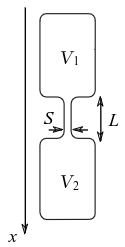
\includegraphics[width = 0.10\textwidth]{V1V2.png}
    \caption{}
\end{wrapfigure}

Для исследования взаимной диффузии газов и
измерения коэффициента взаимной диффузии D используется два сосуда
объёмами $V_1$ и $V_2$ ($V_1 \approx V_2 = V$), соединенные трубкой длины L и 
сечения $S$ (рис. 1). Предполагается, что сосуды заполнены смесью двух газов
при одинаковом давлении, но с различной концентрацией компонентов.

Предположим, что концентрации примеси (гелия) на торцах трубки поддерживаются постоянными и
равными $n_1$ и $n_2$ соответственно. Тогда через некоторое
время в трубке установится стационарный поток частиц, одинаковый в
каждом сечении трубки (в противном случае, если бы поток зависел от $x$,
частицы бы накапливались в трубке, и процесс перестал бы быть стационарным).
Применяя закон Фика в трубке, получим

\begin{equation}
    j = -D \frac{\partial n}{\partial x} = const
\end{equation}

\newpage

Значит, распределение концентрации в трубке $n(x)$ - линейная функция:

\begin{equation}
    n(x) = \frac{\Delta n}{L} \cdot x,
\end{equation}

А плотность потока постоянна:
\begin{equation}
    j = -D \frac{\Delta n}{L}
\end{equation}

Считая процесс квазистатическим, запишем определение плотноти потока:
\begin{equation}
    \frac{dN_1}{dt} = j S, \qquad \qquad \frac{dN_2}{dt} = -j S
\end{equation}

Выразим отсюда скорость изменения $\Delta n$. Вычитая из второго равенства
первое и деля результат на объём сосуда V , с учетом (6) получим

\begin{equation}
    \frac{d \left( \Delta n \right)}{dt} = - \frac{\Delta n}{\tau},
\end{equation}
где $\tau = \frac{1}{D} \frac{VL}{2S}$ для удобства.

Интергрируя выражение (8), получаем, что разность концентраций
будет убывать по экспоненциальному закону

\begin{equation}
    \Delta n = \Delta n_0 e^{-t/\tau}, 
\end{equation}
где $\Delta n_0$ — разность концентраций примеси в сосудах в начальный момент
времени. Видно, что величина $\tau$ есть характерное время выравнивания
концентраций между сосудами. Оно определяется геометрическими размерами
установки и коэффициентом диффузии.

Отметим, что для применимости квазистационарного приближения необходимо
убедиться, что время процесса $\tau$ много больше характерного
времени диффузии отдельной частицы вдоль трубки $L$, которое согласно
закону Эйнштейна–Смолуховского по порядку величины равно
\begin{equation}
    \tau_\text{диф} \sim \frac{L^2}{2 D}
\end{equation}

Таким образом, необходимо выполнение неравенства $\tau \gg \tau_\text{диф}$,
что с учётом (8) и (10) может быть переписано как $SL \ll V$, то есть объём трубки должен
быть много меньше объёма сосудов.

\subsection{Методика измерений}

Для измерения разности концентраций в
установке применяются датчики теплопроводности. При этом используется
тот факт, что теплопроводность $k$ смеси зависит от её состава. При малой разности $\Delta n$
концентраций в сосудах можно ожидать, что разность теплопроводностей будет
изменяться прямо пропорционально $\Delta n$:

\begin{equation}
    \Delta k = k(n_2) - k(n_1) \approx const \cdot \Delta n
\end{equation}

Сами датчики теплопроводности устроены следующим образом. Тонкая
платиновая проволочка, протянутая вдоль оси стеклянного цилиндра,
нагревается током. Внутренняя полость датчика сообщается с объёмом
камеры через отверстия, размеры которых таковы, что скорость диффузии
из объёма сосуда в полость датчика значительно больше скорости диффузии
из одного объёма в другой. Тепло от проволочки к стенке
цилиндра передаётся главным образом за счёт теплопроводности газа, находящегося
внутри цилиндра. При заданной мощности нагревания приращение
температуры проволочки и, следовательно, приращение её сопротивления
пропорциональны теплопроводности газа.

Для измерения сопротивлений используется мостовая схема, позволяющая
определять разность показаний датчиков с высокой точностью.
Мост балансируется при заполнении сосудов одной и той же
смесью. При заполнении сосудов смесями различного состава возникает
«разбаланc» моста. При незначительном различии в составах смесей показания
вольтметра, подсоединённого к диагонали моста, будут пропорцио-
нальны разности концентраций примеси: $U \propto \Delta k \propto \Delta n$. В процессе
диффузии разность концентраций убывает по закону (9), и значит по тому
же закону изменяется напряжение:

\begin{equation}
    U = U_0 e^{-t/\tau}
\end{equation}

где $U_0$ — показание гальванометра в начальный момент времени.

Измеряя экспериментально зависимость $U(t)$, можно получить характерное время
процесса $\tau$, откуда по формуле (8) определить коэффициент диффузии $D$.

\newpage
\section{Экспериментальная установка}

\begin{wrapfigure}{l}{0.5\textwidth}
    \centering
    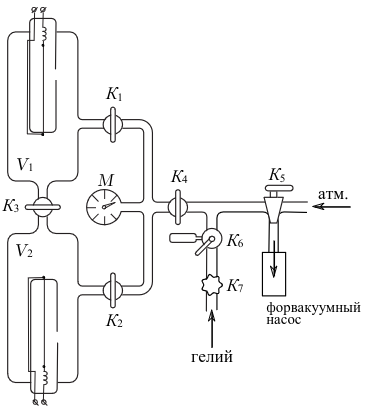
\includegraphics[width = 0.50\textwidth]{ustanovka.png}
    \caption{Экспериментальная установка}
\end{wrapfigure}

Схема измерительной части установки приведена на рис. 2.
Она соединена с системой откачки и напуска воздуха и гелия.
Для откачки используется форвакуумный насос.

Установка компьютеризирована, что позволяет записывать
зависимость показаний вольтметра $U(t)$ в реальном времени

Измерительная часть установки состоит из двух сосудов $V_1$ и $V_2$,
размещённых вертикально. Краны $K_1$ и $K_2$ служат для управления откачкой и
подачей воздуха/гелия в сосуды. Диффузия осуществляется через тонкую
короткую трубку, соединяющую сосуды, оснащённую краном $K_3$.
К соединительным трубкам подключен манометр M,
измеряющий разность давлений между соединительными трубками и атмосферой,
и позволяющий измерять давления в разных частях системы (в зависимости от положения
кранов).
Выравнивание давлений в сосудах $V_1$ и $V_2$ без изменения состава газов в
них может быть осуществлено через обводные трубки
посредством кратковременного открытия кранов $K_1$ и $K_2$ (при закрытом $K_3$)

Датчики теплопроводности, расположенные в сосудах $V_1$ и $V_2$ соответственно,
включены в мостовую электрическую схему согласно рис. 3.

В одну из диагоналей
моста включён высоко-
чувствительный вольтметр (гальванометр) Г,
к другой подключается источник небольшого постоянного
напряжения. Сопротивления проволок датчиков
составляют одно из плеч моста. Второе
плечо составляют переменные сопротивления
$R_1$, $R_2$ и $R$, служащие для установки показаний
вольтметра Г на нуль (балансировка моста).
Сопротивления $R_1$ и $R_2$ спарены (их подвижные контакты находятся
на общей оси) и изменяются одновременно при повороте ручки грубой
регулировки. Точная балансировка выполняется потенциометром $R$.
Балансировку необходимо проводить перед каждым экспериментом заново: при
этом установка заполняется чистым газом (воздухом без гелия) при давлении,
близком «рабочему» (при котором затем будут проводится измерения).

\begin{figure}[h!]
    \centering
    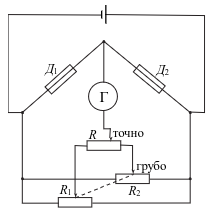
\includegraphics[width = 0.25\textwidth]{most.png}
    \caption{Мост}
\end{figure}

\newpage
\section{Обработка результатов}

\begin{figure}[!htb]
\minipage{0.49\textwidth}
  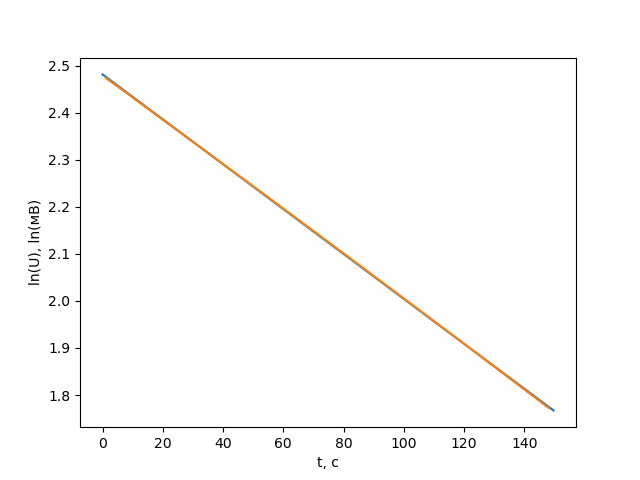
\includegraphics[width=\linewidth]{40.9.png}
  \caption{$P = 40.9$ торр}
\endminipage\hfill
\minipage{0.49\textwidth}
  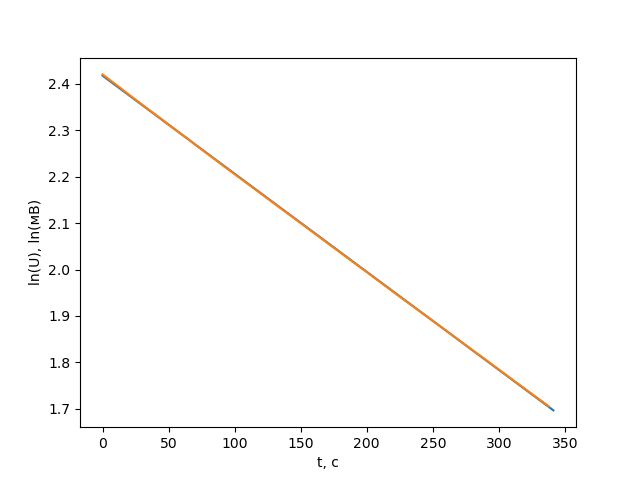
\includegraphics[width=\linewidth]{102.1.png}
  \caption{$P = 102.1$ торр}
\endminipage\hfill
\end{figure}

\begin{figure}[!htb]
\minipage{0.49\textwidth}
  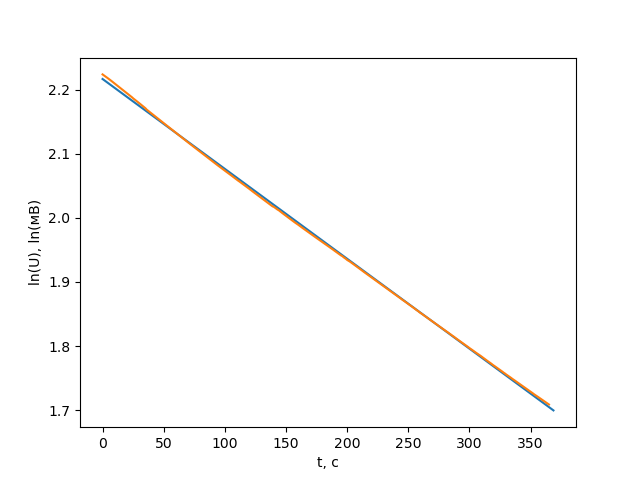
\includegraphics[width=\linewidth]{159.png}
  \caption{$P = 159.0$ торр}
\endminipage\hfill
\minipage{0.49\textwidth}
  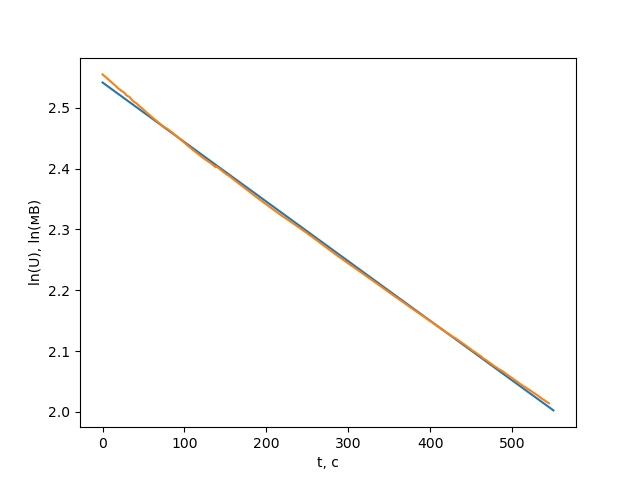
\includegraphics[width=\linewidth]{218.2.png}
  \caption{$P = 218.2$ торр}
\endminipage\hfill
\end{figure}

Подставив коэффициент наклона $k$ в формулу (8), получим:

\begin{equation*}
    D_1 = (9.8 \pm 0.2) \ \frac{\text{см}^2}{\text{c}} \qquad \qquad D_2 = (4.3 \pm 0.1) \ \frac{\text{см}^2}{\text{c}}
\end{equation*}
\begin{equation*}
    D_3 = (2.88 \pm 0.06) \ \frac{\text{см}^2}{\text{c}} \qquad \qquad D_4 = (2.01 \pm 0.04) \ \frac{\text{см}^2}{\text{c}}
\end{equation*}

Теперь построим график $D(\frac{1}{P})$ и экстраполируем до $P_\text{атм}$:

\begin{equation}
    D(P_\text{атм}) = (0.55 \pm 0.2) \ \frac{\text{см}^2}{\text{с}}
\end{equation}

\begin{figure}[h!]
    \centering
    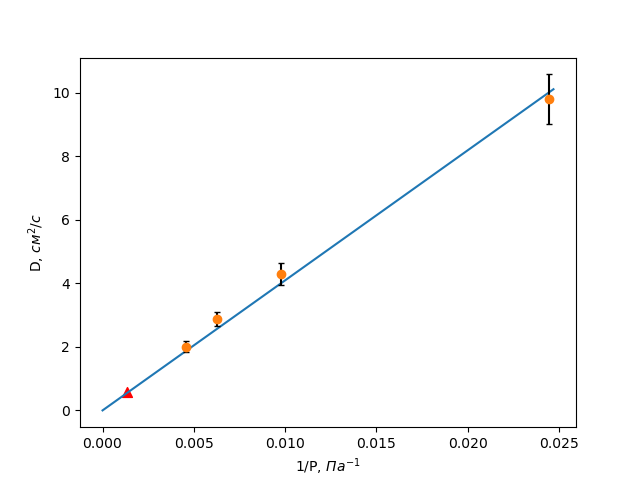
\includegraphics[width = 0.75\textwidth]{D_P.png}
    \caption{Зависимость D(1/P)}
\end{figure}

Оценим также длину свободного пролета и размера молекулы, используя формулу (3).

\begin{equation}
    \lambda = 3 D \sqrt{\frac{\pi \mu}{8RT}} = (1.37 \pm 0.05) \cdot 10^{-7} \ \text{м}
\end{equation}

И эффективное сечение столкновений атомов гелия:

\begin{equation}
    \sigma = (3.0 \pm 0.2) \cdot 10^{-19} \ \text{м}^2
\end{equation}

\newpage

\section{Вывод}

Мы определили коэффициент диффузии гелия в воздухе при разных давлениях,
а также экстраполировали результат до атмосферного давления,
который совпал с табличным в пределах погрешности

\begin{equation*}
    D(P_\text{атм}) = (0.55 \pm 0.2) \ \frac{\text{см}^2}{\text{с}} \qquad \qquad D_\text{табл}(P_\text{атм}) = 0.57 \ \frac{\text{см}^2}{\text{с}}
\end{equation*}

А также мы определили длину свободного пролета молекулы гелия и эффективное сечение
столкновений атомов гелия:

\begin{equation}
    \lambda = (1.37 \pm 0.05) \cdot 10^{-7} \ \text{м}
\end{equation}

\begin{equation}
    \sigma = (3.0 \pm 0.2) \cdot 10^{-19} \ \text{м}^2
\end{equation}

\end{document}
